\documentclass{article}

% If you're new to LaTeX, here's some short tutorials:
% https://www.overleaf.com/learn/latex/Learn_LaTeX_in_30_minutes
% https://en.wikibooks.org/wiki/LaTeX/Basics

% Formatting
\usepackage[utf8]{inputenc}
\usepackage[margin=1in]{geometry}
\usepackage[titletoc,title]{appendix}
\usepackage{authblk}
\usepackage{hyperref}
\hypersetup{
    colorlinks=true,
    linkcolor=blue,
    filecolor=magenta,      
    urlcolor=blue,https://www.overleaf.com/project/5fe04eea6b866846932a22db
}
\documentclass{article}
\usepackage{graphicx}
\graphicspath{ {./images/} }
\urlstyle{same}
% Math
% https://www.overleaf.com/learn/latex/Mathematical_expressions
% https://en.wikibooks.org/wiki/LaTeX/Mathematics
\usepackage{amsmath,amsfonts,amssymb,mathtools}
\usepackage{tikz}

\newcommand{\norm}[1]{\left\lVert#1\right\rVert}
\newcommand*\circled[1]{\tikz[baseline=(char.base)]{
            \node[shape=circle,draw,inner sep=2pt] (char) {#1};}}
\newcommand{\RomanNumeralCaps}[1]
    {\MakeUppercase{\romannumeral #1}}
% Images
% https://www.overleaf.com/learn/latex/Inserting_Images
% https://en.wikibooks.org/wiki/LaTeX/Floats,_Figures_and_Captions
\usepackage{graphicx,float}

% Tables
% https://www.overleaf.com/learn/latex/Tables
% https://en.wikibooks.org/wiki/LaTeX/Tables

% Algorithms
% https://www.overleaf.com/learn/latex/algorithms
% https://en.wikibooks.org/wiki/LaTeX/Algorithms
\usepackage[ruled,vlined]{algorithm2e}
\usepackage{algorithmic}

% Code syntax highlighting
% https://www.overleaf.com/learn/latex/Code_Highlighting_with_minted
\usepackage{minted}
\usemintedstyle{borland}

% References
% https://www.overleaf.com/learn/latex/Bibliography_management_in_LaTeX
% https://en.wikibooks.org/wiki/LaTeX/Bibliography_Management
\usepackage{biblatex}
\addbibresource{references.bib}

%theorems
\usepackage[utf8]{inputenc}
\usepackage[english]{babel}

\usepackage{amsthm}
\newtheorem{theorem}{Theorem}[section]
\newtheorem{lemma}[theorem]{Lemma}



% Title content
\title{Final Project\\
Learning Contextual Bandits with Missing Rewards}
\author{Shahar Peleg, Omri Manor, Orin Levy }

\affil{\href{mailto:shaharpeleg@mail.tau.ac.il}{shaharpeleg@mail.tau.ac.il}, \href{mailto:omrimanor@mail.tau.ac.il}{omrimanor@mail.tau.ac.il}, \href{mailto:orinlevy@mail.tau.ac.il}{orinlevy@mail.tau.ac.il}}
\begin{document}
\maketitle

% Abstract
\section{Abstract}

In this project, we will consider the Contexual Multi Arm Bandit model, where some of the rewards won't be available to the learner (“missing rewards”). This setting is motivated by real-life scenarios that match the online learning setting.\\


Our goal is to present algorithms in which the learner can make use the context in order to learn, even if the reward is missing. At first, for comparison, we will present a naive LinUCB algorithm that simply ignores the context when the reward is missing and analyse it. Then, we will show different approaches to approximate the reward when missing. We will take advantage of the fact that the expected reward of each arm is a linear function of the context.\\

In this project we will present two algorithms, Cover Approximated LinUCB and an improvement of MLinUCB algorithm presented by Bouneffouf, Upadhyay and Khazaeni in [4]. In Cover ALinUCB, we use balls (with predetermined radius) to cover the context space (we will assume it is a compact set). We will use the fact that the difference between rewards of every two contexts in the same ball is bounded by the diameter of the ball. By using this method we achieved expected regret $R(T) = \Tilde{O}(\sqrt{T}(\sqrt{M} + \sqrt{d}))$ where $M$ bound the bound the number of missing rewards and $d$ is the contexts space dimension. \\

We also show an empirical improvement of the MLINUCB algorithm[4], which uses unsupervised learning  algorithm (clustering) to address those missing rewards. We propose to use an optimal number of clusters in the algorithm, by using the Elbow method. By doing that, the agent learns better from the data, even if the reward is missing. We will introduce an algorithm that use the optimal number of clusters, $N$, instead of having it as a given input for the model. We will show that the algorithm performs better on a real-life dataset. As the Elbow method is heuristic with no established results, we will only show experimental results in that section. 
% Introduction
\section{Introduction and Motivation}

The multi-armed bandit problem (MAB) is a classic online learning problem where an agent makes decisions over time under uncertainty. We are given a slot machine with $K$ arms (bandits), where each arm having its own probability distribution of success. Pulling any one of the arms gives you a stochastic reward. Our objective is to pull the arms one-by-one in sequence such that we maximize our total reward collected in the long run (or to minimize the regret). The MAB problem exemplifies the exploration–exploitation tradeoff dilemma. \\

A particularly useful version of the multi-armed bandit is the contextual multi-armed bandit problem. In this problem, in each iteration an agent has to choose between arms. Before making the choice, the agent sees a d-dimensional feature vector (context vector), associated with the current iteration. The learner uses these context vectors along with the rewards of the arms played in the past to make the choice of the arm to play in the current iteration. Over time, the learner aims to collect enough information about how the context vectors and rewards relate to each other, so that it can predict the next best arm to play by looking at the feature vectors[2].\\

We will consider a novel variant of the contextual bandit problem (where each round the decision-maker is exposed to extra side-information, which is the context). In this variant, the reward associated with each context-based action choice may not always be observed after making the decision. This setting is motivated by several online settings such as clinical trials and ad recommendation applications, where the outcome of each decision may not always be revealed immediately to the learner.\\

\section{Problem Setting}

Let $C \subseteq \mathbf{R}^d$ be the context space such that $\norm{x_t} \leq 1$. $x_t \in C$ is the context at time $t$, $r_{t,i}\in [0,1]$ is the reward of action $i$ at time $t$ and $r_t \in [0,1]^K$ denotes a vector of rewards at time $t$.\\
We will assume there is a joint probability distribution $D_{c,r}$ over $(x,r)$. $A= \{1,2,..,K\}$ will be the set of actions and $\pi:C\rightarrow A$ denotes a policy. We will assume there exist an unknown weights matrix $\theta^* \in \mathbf{R}^{d\times k}$, $\|\theta^*\|\leq 1$ such that :
\[\forall k,t:\quad \mathbf{E}[r_k(t)|x_t]= \theta^\top_kx_t\]
Where $\theta_k \in \mathbf{R}^d$ is an unknown coefficient vector associated with arm $k$ which needs to be learned from the data. Hence, we assume that $r_{t,k}$ are independent random variables with expectation $x^\top\theta^*_k $.\\

Our benchmark is 
\[R(T) = \sum_{t=1}^T r_{t,k^*(t)} - \sum_{t=1}^T r_{t,k(t)}\]
where $k^*(t) = \arg\max_{k} \{x^T_t \theta^*\}$ is the best action for the context at time $t$ according to $\theta^*$.\\


% Related work
\section{Related work}

Contextual bandit with linear rewards model, in the case where there is no missing data, is solved in two papers, (Chu et al [6], Abbasi-Yadkori et al [7]). In our work, we will refer to the version presented in [6], and adapt it to our settings. LinUCB algorithm presented in [6] solves it with a regret of $\Tilde{O}(\sqrt{dT})$, using the technique of Online Ridge Regression. Note that the general CBP setting ([6],[7]) takes one context per arm instead for our setting of the one context share by actions.\\

In our work, we use the LinUCB algorithm, and approximating the missing reward with several techniques. We were inspired from Cover-RMAX presented in [5], where the method of balls covering for the context space is presented.\\

In addition, our work will be based on [4] too. In this paper, the MLinUCB algorithm is presented, where they use an unsupervised learning method such as clustering to handle the missing rewards. The regret of the MLinUCB algorithm with probability $1-\delta$ is:

$$ R(T) \leq \sigma \Bigg( \sqrt{d \log(\frac{\det(A_T)^{0.5}}{\delta \det(S)^{0.5}})} + \frac{\norm{\theta}}{\sqrt{\phi}} \Bigg) \sqrt{18 T \log(\frac{\det(A_T)}{\det(S)})}$$

with $\phi \in \mathbf{R}$, $\norm{x_t}_2 \leq L$, $S = I_d + \sum _{t \in s} x_tx_t^T$ where $s \subseteq T$ contains the times where the context is with missing reward and 
$A_T = S + \sum _{t \notin S} x_t x_t^T$. Note that the matrix $A_T$ represents all the context vectors, whereas the matrix $S$ represents only the missing ones. In addition, the regret has a linear ratio in the number of the missing rewards. Taking a look on $A_T$ and $S$, both has a linear dependency in the contexts with missing rewards, which is expressed in the regret by their determinants.\\
In their model, they are assuming:
\[\forall k,t:\quad \mathbf{E}[r_k(t)|x_t]= \theta^\top_kx_t +n_t\]
where $n_t$ is independent $\sigma-sub-Gaussian$ noise, which yields the factor of $\sigma$ in the above regret. In our model, we omitted the sub-gaussian noise, as our analysis is based on [6], where no noise was considered.

\section{Naive LinUCB - assuming up to $M$ missing rewards}

\subsection{The Setting}
We will assume the described setting, and in addition that the number of rounds in which the learner will see no reward after playing the chosen action is bounded by $M$, a pre-determined constant.\\
In those $M$ rounds the presented algorithm will ignore the context we see. \\

\subsection{The Algorithm}

\begin{algorithm}[H]
\SetAlgoLined
 \textbf{Input:} value for $\alpha, b_0, \textbf{A}_0$ \\
 \For {$t = 1$ to $T$}{

    \For {all $k \in K$}{  
    $\theta_k \gets \textbf{A}_{k_t}^{-1} * b_{k_t}$ \\
    $p_{t,k} \gets  \theta_k^\top x_t + \alpha \sqrt{x_t^\top \textbf{A}_{k_t}^{-1} x_t}$
    }
    choose arm $k_t = argmax_{k \in K} p_{t,k}$, and observe real-valued payoff $r_t$\\ 
    \eIf {$r_t$ available}
    {retrieve $r_t$ from data}{continue}
    
    $\textbf{A}_{k_t} \gets \textbf{A}_{k_t} + x_{t,k_t}x_{t,k_t}^\top$\\
    $b_{k_t} \gets b_{k_t} + r_t x_{t,k_t}$
    }
    
 \caption{Naive Missing LinUCB}
\end{algorithm}

\subsection{Regret analysis}
\subsubsection{Theorem}

With probability $1- \delta$ we have: 
$$ R(T) \leq \Tilde{O} ( M + \sqrt{dT} ) $$

\subsubsection{Proof of theorem}
In the $T-M$ rounds where we observe the rewards, we will operate as in LinUCB (and suffer LinUCB regret, $\Tilde{O} (\sqrt{dT})$), while in the other $M$ rounds we assume maximal loss of 1 for each round. Thus, the overall regret is as stated above.

\subsection{Conclusion}
The above naive version of LinUCB ignores contexts with missing rewards, and hence learning in only $T-M$ rounds, in the worst case. In the following presented algorithm, we will try to take advantage of the fact that the expected reward of each arm is a linear function of the context, and approximate the missing reward.

\section{Cover Approximated LinUCB}

We will try a different approach for approximating the missing rewards, while using context space covering.
We chose to use balls covering of the context space.\\
Utilizing the assumption that our context space $C$ is a compact set, we can create a cover of $C$ with finitely many balls $B_{\gamma_0}(o_i)$ of radius $\gamma_0$ centered at $o_i \in \mathbf{R}^d$.
The size of the cover, i.e., the number of balls, can be measured by the notion of covering numbers, defined as
$$ N(C,\gamma_0) = \min\{|Y|: C \subseteq \cup_{y \in Y} B_{\gamma_0}(y)\} $$
The algorithm receives $B=\{o_i\}_{i=1}^N$ and the radius $\gamma_0$ as an input.\\

Let $R_{b_i}(a)$ denote the total reward obtained from action $a$ for contexts inside the $i$-th ball $b_i=(o_i,\gamma_0)$.\\
Let us define the approximated reward of missing contexts which belong to the ball $b_i$ to be:
$$ \hat{r}_{b_i}(a) = \frac{R_{b_i}(a)}{n_{b_i}(a)}$$
where $n_{b_i}(a)$ is the number of samples of contexts inside the ball and their related rewards for action $a$.
For a context $x_t$ with no reward, we will use $\hat{r}_{b_i}$ as the reward, where $b_i$ is the ball where $x_t$ lays.\\

Our intuition is that for every two contexts in the same ball, their expected reward for each arm is similar, as the reward of each arm is an inner product. Thus, the optimal choice of action for these contexts might be similar as well. We can assume that for each ball, when the algorithm sees a missing reward, there is already enough data from contexts in the ball for the $\hat{r}_{b_i}(a)$ calculation. Therefore, we will assume that we can calculate  $\hat{r}_{b_i}(a)$ when the reward is missing. We propose to use a ball with a constant radius instead of using KNN and K-means. This because in high dimensional spaces those methods can cause two very different vectors to sit under the same cluster. Using balls lets us bound the distance between different vectors in the same subset which is used to approximate the missing rewards.\\

\subsection{The Algorithm:}

\begin{algorithm}[H]
\SetAlgoLined
 \textbf{Input:} value for $\alpha, b_0, \textbf{A}_0, B=\{o_i\}_{i=1}^N, \gamma_0$ \\
 \For {$t = 1$ to $T$}{

    \For {all $k \in K$}{  
    $\theta_k \gets \textbf{A}_{k_t}^{-1} * b_{k_t}$ \\
    $p_{t,k} \gets  \theta_k^\top x_t + \alpha \sqrt{x_t^\top \textbf{A}_{k_t}^{-1} x_t}$
    }
    choose arm $k_t = argmax_{k \in K} p_{t,k}$, and observe real-valued payoff $r_t$\\ 
    \eIf {$r_t$ available}
    {retrieve $r_t$ from data}
    {set $r_t = \hat{r}_{b_i}(k_t)$ for ball $b_i$ such that $x_t \in b_i$}
    
    $\textbf{A}_{k_t} \gets \textbf{A}_{k_t} + x_{t,k_t}x_{t,k_t}^\top$\\
    $b_{k_t} \gets b_{k_t} + r_t x_{t,k_t}$
    }
    
 \caption{Cover Approximated LinUCB}
\end{algorithm}

\subsection{Analysis}
\begin{lemma}
Let $x_1, x_2 \in C$ be two different contexts which lays in the same ball, namely $x_1, x_2 \in B_{\gamma_0}(o_i)$, then we have for every action $k$:
\begin{equation}
    \norm{x_1^\top \theta^*_k - x_2^\top \theta^*_k} \leq 2\gamma_0
\end{equation}

\end{lemma}

\begin{proof}
    As $\norm{\theta_k} \leq 1$ and since $x_1,x_2$ are in the same ball, we have $\norm{x_1^T - x_2^T} \leq 2\gamma_0$ and by Cauchy–Schwarz inequality we have
    \begin{equation}
      \norm{x_1^\top \theta^*_k - x_2^\top \theta^*_k} =  \norm{(x_1^\top- x_2^\top)\theta^*_k} \leq \norm{x_1^\top- x_2^\top}\norm{\theta^*_k} \leq \norm{x_1^\top- x_2^\top} \leq 2\gamma_0  
    \end{equation}
\end{proof}

\begin{lemma}
For every two contexts $x_{t_1}, x_{t_2}$ which lay in the same ball, and have been seen in time steps $t_1, t_2$ of the algorithm's run:
\begin{equation}
    \begin{split}
        |\mathbf{E}[r_k(t_1) - r_k(t_2)|x_{t_1},x_{t_2}]| 
        &\leq 2 \cdot \gamma_0
    \end{split}
\end{equation}
\end{lemma}

\begin{proof}
Since for every time step $t$ and arm $k$ we have $\mathbf{E}[r_k(t)|x_t] = \theta_k^{\top} \cdot x_t$ then:
 \begin{equation}
    \begin{split}
        |\mathbf{E}[r_k(t_1) - r_k(t_2)|x_{t_1},x_{t_2}]| = |\theta^\top_k \cdot x_{t_1} - \theta^\top_k \cdot x_{t_2}| \underbrace{\leq}_{\text{Lemma  6.1}} 2 \cdot \gamma_0
    \end{split}
\end{equation}
\end{proof}

\begin{lemma}

Let $x_t$ be the context at time $t$ and assume a reward $r_t$ was not available to the learner (in time $t$). Assume the played action in time $t$ was $k_t$ and $x_t \in B_{\gamma_0}(o_i)$. Then,
$$ \norm{r_t - \hat{r}_{b_i}(k_t)} \leq 2 \gamma_0 $$
\end{lemma}

\begin{proof}
Denote $I = \{0 \leq \tau < t \ | \ x_{\tau}\in B_{\gamma_0}(o_i) \text{, the played action was $k_t$ and the reward seen was } r_{\tau} \}$, then we have:
\begin{equation}
    \begin{split}
        \norm{r_t - \hat{r}_{b_i}(k_t)} &\leq \norm{r_t - \frac{\sum_{\tau \in I} r_{\tau}}{|I|}}\\
        &\leq |\frac{r_t|I| - \sum_{\tau \in I} r_{\tau}}{|I|}|\\
        &\leq |\frac{\sum_{\tau \in I} (r_{\tau}-r_t)}{|I|}|\\
        &\text{and by Lemma 6.2} \\
        &\leq \frac{2\gamma_0 \cdot |I|}{|I|}\\
        &= 2 \gamma_0
    \end{split}
\end{equation}
\end{proof}


\begin{theorem}
With probability $1-\delta$ the regret bound of the Cover Approximated LinUCB algorithm is:
$$ R(T) \leq  \Tilde{O}(\sqrt{Td} + \sqrt{M}) $$
\end{theorem}


\begin{proof}
Let $x_t \in C$ be the context vector in time $t$ and let $R(t)$ be the regret suffered in time $t$. Then:
\begin{equation}
    \begin{split}
        R(t) = \norm{x^\top_t \theta^*_{k^*_t} - x^\top_t \theta^ t _{k_t}} = \norm{x^\top_t\theta^*_{k^*_t} + x^\top_t \theta^ \ell _t - x^\top_t \theta^ \ell _t - x^\top_t \theta^t _{k_t}}_2
    \end{split}
\end{equation}

where $k^*_t = \arg \max _k {x^\top_t \theta _k ^*}$,$k_t$ is the action played in time $t$ and $\theta ^ \ell$ is the parameter learned in LinUCB algorithm as presented in [6].  $\theta^t _{k_t}$ is the parameter learned by Cover Approximated LinUCB algorithm at time $t$ and we will denote it as $\theta _t$.\\
Using the triangle inequality we get:

\begin{equation}
    \begin{split}
        R(t) \leq \underbrace{ \norm{x^\top_t\theta^*_{k^*_t}  - x^\top_t \theta^ \ell _t }_2}_{\alpha_t} + \underbrace{ \norm{x^\top_t \theta^ \ell _t - x^\top_t \theta^t _{k_t}}_2}_{\beta_t}
    \end{split}
\end{equation}
Now, 
\begin{equation}
   R(T) \leq \sum_{t=1}^T \alpha_t + \beta_t = \sum_{t=1}^T \alpha_t + \sum_{t=1}^T \beta_t
\end{equation}
where with probability $1-\delta$ we have:
\begin{equation}
    \sum_{t=1}^T \alpha_t \leq \Tilde{O}(\sqrt{dT})
\end{equation}
as this is exactly the regret of LinUCB as analysed by Chu et al [6].\\
Now we will bound the $\beta_t$ expression:

\begin{equation}
    \begin{split}
        \beta_t = \norm{x_t ^\top \theta_t^\ell - x_t^\top \theta_t} = \norm{x_t ^\top A^{-1}_t b_t - x_t ^\top A^{-1}_t \hat{b}_t} \leq \norm{x_t ^\top A^{-1} _t}\cdot\norm{b_t-\hat{b}_t}
    \end{split}
\end{equation}

Where by the update rule of LinUCB we have $\theta^\ell _t = A^{-1} _t b_t $ and $b_t = \sum_{t=1}^T r_t x_t$.\\
Let us denote by $S_t$ the set of time steps where there was no reward available until time $t$, then by Cover Approximated LinUCB's update rule we have $\theta _t = A^{-1} _t \hat{b}_t $ where $\hat{b}_t = \sum_{t \notin S_t} r_t x_t + \sum_{t \in S_t} \hat{r}_t x_t$.\\
Note that the matrices $A_t$ are identical in both algorithms. \\

We will bound each expression separately,

\begin{equation}
    \begin{split}
        \norm{b_t-\hat{b}_t} &= \norm{\sum_{\tau=1}^t r_{\tau} x_{\tau} -  \sum_{\tau \notin S_t} r_{\tau} x_{\tau} - \sum_{\tau \in S_t} \hat{r}_{\tau} x_{\tau}}\\
        &= \norm{\sum_{\tau \in S_t} (r_{\tau}- \hat{r}_{\tau}) x_{\tau}}\\
         &\text{and by Lemma 6.3} \\
        &\leq 2\gamma_0 \cdot \norm{\sum_{\tau \in S_t} x_\tau}\\
        &\leq 2\gamma_0 M_t
    \end{split}
\end{equation}
Where $M_t = |S_t|$.\\

Using the proof of Lemma 1 in [6], by the same calculations we get:
\begin{equation}
    \begin{split}
        \norm{x_t ^\top A^{-1} _t}_2 \leq \norm{x_t}_{A_t^{-1}}
    \end{split}
\end{equation}
Therefore,
\begin{equation}
    \begin{split}
        \beta_t  \leq \norm{x_t ^\top A^{-1} _t}\cdot\norm{b_t-\hat{b}_t} \leq \norm{x_t}_{A_t^{-1}} \cdot  2\gamma_0 M_t
    \end{split}
\end{equation}

As $M$ upper bounded the total number of missing rewards, and $T$ is total time steps.\\
All the norms are equal, therefore for every two norms $n_1, n_2$ there exists $z,Z > 0$ such that $\forall v \in R^d$ we get:
$$z \norm{v}_{n_2} \leq \norm{v}_{n_1}  \leq Z \norm{v}_{n_2}$$\\
Thus, for all $t$ there exists $z_t$ such that $\norm{x_t}_{A_t^{-1}} \leq z_t \norm{x_t}_2$. We will choose $z = \max\limits_{t} z_t$ and get as $\norm{x_t} \leq 1$:
\begin{equation}
    \begin{split}
        \beta_t \leq 2\gamma_0 M z
    \end{split}
\end{equation}
Now,
\begin{equation}
  \sum_{t=1}^T \beta_t \leq 2 \gamma_0 MzT
\end{equation}
By setting $\gamma_0 = \frac{1}{T\sqrt{M}}$, and for appropriate set of centers $B= \{o_i\}_{i=1}^N$ we will have: 
\begin{equation}
  \sum_{t=1}^T \beta_t \leq 2z\sqrt{M}
\end{equation}
Overall we get, with probability $1-\delta$:
\[R(T) \leq \Tilde{O}(\sqrt{Td}) +  2z\sqrt{M}  = \Tilde{O}(\sqrt{Td}+\sqrt{M})\]
\end{proof}

\section{MLINUCB and optimal number of clusters}

The researchers in [4] adapted the LinUCB algorithm, proposing to use a clustering step for estimation of the reward data when it's missing. At each time step, they added a clustering step on the context vectors where the total number of clusters $N$ is a hyperparameter. For each cluster $j$ they defined the average reward for each arm as below:

\[\bar{r_j} = \frac{\sum_{\tau=1}^{n_j} r_\tau}{n_j}\]
Assuming $d_j = dist(x_t, \gamma_j)$ is the metric used for clustering where $\gamma_j$ is the $j^{th}$ cluster centroid and $n_j$ is the number of data points in cluster $j$, the $m$ smallest $d_j$ are chosen as the closest clusters to $x_t$ and a weighted average of the average cluster rewards is computed by:\\

\[g(x_t) = \frac{\sum_{j=1}^m \frac{\bar{r_j}}{d_j}}{\sum_{j=1}^m \frac{1}{d_j}}\]
When $r_t$ is missing, $r_t = g(x_t)$ is assigned. Note that if $m = 1$, $g(x_t)$ is simply the average rewards of all the points within the cluster that $x_t$ belongs to.\\

\begin{algorithm}[H]
\SetAlgoLined
 \textbf{Input:} value for $\alpha, b_0, \textbf{A}_0, m, N$ \\
 \For {$t = 1$ to $T$}{
    cluster \{$x_1, ... , x_t$\} into $N$ clusters\\
    \For {all $k \in K$}{  
    $\theta_k \gets \textbf{A}_{k_t}^{-1} * b_{k_t}$ \\
    $p_{t,k} \gets  \theta_k^\top x_t + \alpha \sqrt{x_t^\top \textbf{A}_{k_t}^{-1} x_t}$
    }
    choose arm $k_t = argmax_{k \in K} p_{t,k}$, and observe real-valued payoff $r_t$\\ 
    \eIf {$r_t$ available}
    {retrieve $r_t$ from data}
    {$r_t \gets g(x_t)$}
    
    $\textbf{A}_{k_t} \gets \textbf{A}_{k_t} + x_{t,k_t}x_{t,k_t}^\top$\\
    $b_{k_t} \gets b_{k_t} + r_t x_{t,k_t}$
    }
    
 \caption{MLinUCB}
\end{algorithm}\\
Note: successful MLinUCB operates on the assumption that the context vectors live in a manifold that can be described by a set of clusters. Thus, MLinUCB has the potential to outperform LinUCB when this manifold assumption
holds, specifically when the number of clusters chosen adequately describes the structure of the
context vector space.\\


\subsection{Optimal Number of Clusters}
Our goal in this section was to optimize the number of clusters, $N$. In [4], the model was trained with several values of $N$, and the results for each $N$ were compared in order to find the best $N$. \\
Our approach is to achieve high accuracy with a single train of the model, without predetermining the number of clusters $N$ in the model input.\\

We implemented the MLinUCB model and removed the number of clusters as an input. Instead, we added an optimal clustering algorithm, using the Elbow method, in order to achieve better accuracy with a single train of the model.\\

\subsubsection{Elbow Method for Clustering}

K-Means Clustering is a localized optimization method that is sensitive to the selection of the starting position from the midpoint of the cluster. Choosing the starting position from the midpoint of a bad cluster will result in K-Means Clustering algorithm resulting in high errors and poor cluster results. The K-means algorithm has problems in determining the best number of clusters. The Elbow method looks for the best number of clusters on the K-means method. By using the elbow method, we can optimize the results of our model, and choose the best number of clusters on each iteration, to maximize the accuracy.\\
Note that the Elbow method is heuristic with no established theoretical results, thus we will use it for the experiments only, and will receive empirical results.\\


\begin{algorithm}[H]
\SetAlgoLined
 \textbf{Input:} value for $\alpha, b_0, \textbf{A}_0, m$ \\
 \For {$t = 1$ to $T$}{
    \For {all $k \in K$}{ 
    $\theta_k \gets \textbf{A}_{k_t}^{-1} * b_{k_t}$ \\
    $p_{t,k} \gets  \theta_k^\top x_t + \alpha \sqrt{x_t^\top \textbf{A}_{k_t}^{-1} x_t}$
    }
    choose arm $k_t = argmax_{k \in K} p_{t,k}$, and observe real-valued payoff $r_t$\\
    \eIf {$r_t$ available}
    {retrieve $r_t$ from data}
    {$N \gets$ Elbow method clustering\\
    cluster \{$x_1, ... , x_t$\} into $N$ clusters\\
    $r_t \gets g(x_t)$}
    
    $\textbf{A}_{k_t} \gets \textbf{A}_{k_t} + x_{t,k_t}x_{t,k_t}^\top$ \\
    $b_{k_t} \gets b_{k_t} + r_t x_{t,k_t}$ }
    
 \caption{MLINUCB with Elbow Method}
\end{algorithm}

\subsection{Results}

We trained the model with 10\%, 50\% and 75\% missing rewards, with different predetermined $N$ parameter values, as well as with the Elbow method, without a given $N$ parameter in the input. We chose to use the CNAE-9 dataset from the UCI Machine Learning Repository, who holds the manifold assumption.\\

In the table below we compare the results of the model accuracy for several values of missing rewards percentage. In the first columns we show the model with a pre-defined number of clusters (2, 5 and 10 clusters), while in the last column we show the results of using the Elbow method.\\

\begin{table}[h!]
\begin{center}
\begin{tabular}{ |c||c|c|c|c| } 
 \hline 
  & N=2 & N=5 & N=10 & Elbow Method\\ 
 \hline \hline
 10\% missing rewards & 0.29 & 0.23 & 0.27 & 0.48\\ 
 \hline
 50\% missing rewards & 0.19 & 0.19 & 0.25 & 0.39\\ 
 \hline
 75\% missing rewards & 0.14 & 0.14 & 0.09 & 0.14\\ 
 \hline
\end{tabular}
\caption{CNAE-9 - Model Accuracy}
\end{center}
\end{table}\\
Following are the graphs of the model training with 10\% and 50\% missing data, showing the accuracy of the model VS the number of events the model seen so far.\\
\begin{figure}[H]
\centering
\begin{subfigure}{\textwidth}
  \centering
  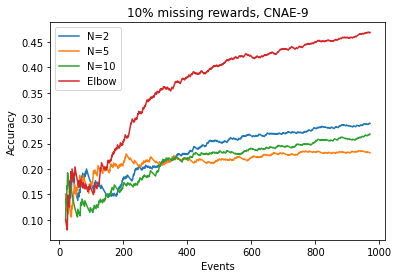
\includegraphics[width=.4\linewidth]{CNAE9, 10 missing}
  \label{fig:sub1}
\end{subfigure}%
\begin{subfigure}{\textwidth}
  \centering
  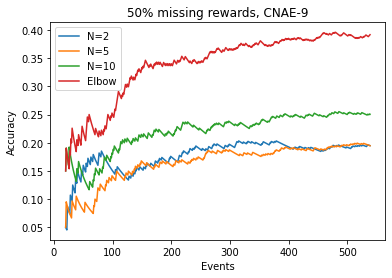
\includegraphics[width=.4\linewidth]{CNAE9, 50 missing2}
  \label{fig:sub2}
\end{subfigure}
\label{fig:test}
\end{figure}\\
As we can see in the table and in the graphs above, the Elbow method mostly got the best accuracy value, or at least the highest accuracy reached with the training that was done with the parameter $N$ given.\\


\section{Summary and Conclusions}
In this project we tried to show different solutions to the problem of missing rewards. We presented several approaches to take advantage of the contexts in order to estimate the missing rewards.\\
The algorithms we've seen so far suffer loss for every missing reward, and don't take advantage of the related context when a reward is missing.\\

We believed that with tighter analysis, we can achieve more significant improvement to those algorithms, as in our approach we can bound how far our approximated reward from the true unrevealed reward, and we can tune this distance.
This in oppose to the MLinUCB algorithm, where they can't bound the distance between their approximation to the true reward. This because they are clustering in high-dimensional space, as explained above. If we could express our regret similar to their regret, using similar matrices, we believe our results were better. \\

In conclusion, our analysis is probably not tight, but we do believe that with a more tight analysis, we can improve the regret before determining $\gamma_0$.

\newpage

\begin{thebibliography}{9}
\bibitem{latexcompanion} 
MA Syakur, BK Khotimah, EMS Rochman and BD Satoto.
\textit{Integration K-Means Clustering Method and Elbow Method For Identification of The Best Customer Profile Cluster}. 
Faculty of Engineering, University of Trunojoyo Madura, 2018.

\bibitem{latexcompanion} 
John Langford, Tong Zhang
\textit{The Epoch-Greedy Algorithm for Contextual
Multi-armed Bandits}. 
Department of Statistics
Rutgers University, 2007.

\bibitem{latexcompanion} 
Lihong Li, Wei Chu, John Langford, Robert E. Schapire
\textit{A Contextual-Bandit Approach to
Personalized News Article Recommendation}. 
2012.

\bibitem{latexcompanion} 
Djallel Bouneffouf, Sohini Upadhyay and Yasaman Khazaeni
\textit{Online learning from Less Data: Contextual Bandit with Missing Rewards}.
IBM Research AI, 2020.

\bibitem{latexcompanion} 
Aditya Modi, Nan Jiang, 
Satinder Singh and Ambuj Tewari
\textit{Markov Decision Processes with Continuous Side Information}.
Algorithmic Learning Theory 2018.

\bibitem{latexcompanion} 
Wei Chu, Lihong Li, 
Lev Reyzin and Robert E. Schapire
\textit{Contextual Bandits with Linear Payoff Functions}.
Proceedings of the Fourteenth International Conference on Artificial Intelligence and Statistics, JMLR Workshop and Conference Proceedings, 2011.

\bibitem{latexcompanion} 
Yasin Abbasi-Yadkori, D´avid P´al, Csaba Szepesv´ari
\textit{Improved Algorithms for Linear Stochastic Bandits}.
University of Alberta, NIPS 2011.

\end{thebibliography}


\end{document}
